\subsection{Computational aspects}
\begin{frame}
    \frametitle{Computational Aspects}
    \framesubtitle{The computational challenge}

    \begin{itemize}
        \item The {\nbody} codes evolution is related to the available
                \blue{hardware} in our time.
        \item The algorithms with a complexity of $O(N^{2})$ or $O(N^{3})$ require
                \red{supercomputers}.
        \begin{itemize}
            \item  e.g \blue{beowulf clusters},
                which require a parallelization of the code
                (\textsc{Nbody6++} developed by Spurzem et al.~\cite{Spurzem1999}).

            \item Special-purpose hardware, like the \blue{GRAPE} (short for GRAvity
                PipE system~\cite{TMFES96,MT98,Makino98,GRAPE6A}.
        \end{itemize}

        \item  The literature overview reveals a strong interest on porting the existing codes to the
            \blue{GPU} architecture, like e.g. the work
            of~\cite{Portegies2007a,Hamada2007,Belleman2008}
            on single nodes or using large
            clusters~\cite{berczik2011high,NitadoriAarseth2012,Capuzzo-DolcettaEtAl2013}.

    \end{itemize}

\end{frame}

\subsubsection{CPU approach}
\begin{frame}
    \frametitle{Computational Aspects}
    \framesubtitle{Parallel CPU implementation}
    \begin{itemize}
        \item Single-core implementation to perform a profiling (\texttt{gprof}).
        \begin{itemize}
            \item Gravitational interaction is the bottleneck.
            \item Usually $N_{act} << N$.
        \end{itemize}
        \item Many-core with OpenMP.
        \begin{itemize}
            \item \soft{\texttt{\#pragma omp parallel for}}
        \end{itemize}
        \item Many-core with MPI (two implementations)
        \begin{itemize}
            \item \soft{\texttt{MPI\_Allreduce, MPI\_Bcast}}
        \end{itemize}
    \end{itemize}
\end{frame}

\begin{frame}[fragile]
    \frametitle{Computational Aspects}
    \framesubtitle{Parallel CPU implementation}

    \begin{columns}
        \begin{column}{0.45\textwidth}
            \begin{lstlisting}[language=C,caption={Reduce every $Nact$ particle}]
for (int i = 0; i < Nact; i++)
{
    ...
    for (int j = 0; j < N; j++)
    {
        gravitational_interaction(...);
    }
    ...
    MPI_Allreduce(...);
}
            \end{lstlisting}
        \end{column}
        \begin{column}{0.45\textwidth}
            \begin{lstlisting}[language=C,caption={Reduce all $Nact$ particle}]
for (int i = 0; i < Nact; i++)
{
    ...
    for (int j = 0; j < N; j++)
    {
        gravitational_interaction(...);
    }
    ...
}
MPI_Allreduce(...);
            \end{lstlisting}
        \end{column}
    \end{columns}
\end{frame}

\subsubsection{GPU Computing}
\begin{frame}
    \frametitle{Computational Aspects}
    \framesubtitle{GPU Computing}

    \begin{columns}
        \begin{column}{0.6\textwidth}
            \begin{center}
                \emph{"Using a GPU (Graphic Processing Unit) together with
                a CPU to accelerate scientific calculation operations
                or general purpose calculation"}
            \end{center}
        \end{column}
        \begin{column}{0.4\textwidth}
             \begin{figure}
                 \centering
                 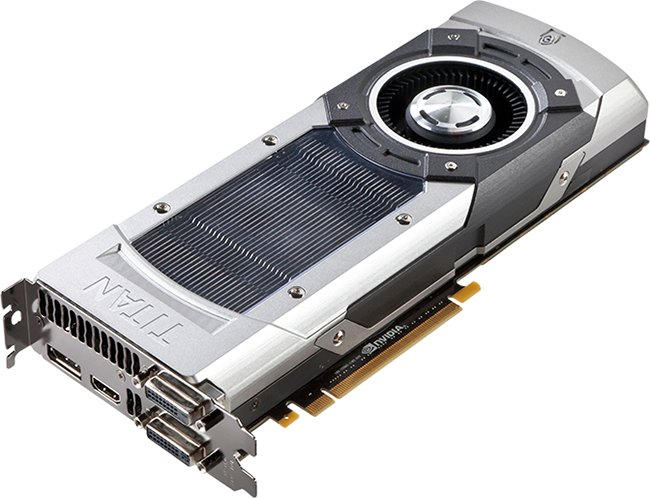
\includegraphics[width=0.8\textwidth]{img/titan}
                 \caption{NVIDIA\textsuperscript{\textregistered} GTX Titan}
                 \label{fig:titan}
             \end{figure}
        \end{column}
    \end{columns}
\end{frame}

\begin{frame}
    \framesubtitle{CPU/GPU Design}

    \begin{itemize}
        \item CPU,
        \begin{itemize}
            \item Designed to have a good \blue{performance}
                  in parallel and non-parallel scenarios.
            \item Minimizes the \blue{latency} experimented by a thread
                  (large cache memory)
        \end{itemize}
        \item GPU,
            \begin{itemize}
            \item Designed to perform highly parallel work.
            \item Maximizes the \blue{throughput} of all the threads.
            \end{itemize}
    \end{itemize}

    \begin{footnotesize}
        \begin{columns}
            \begin{column}{0.35\textwidth}
            \begin{block}{Performance}
                Capacity of perform individual instructions in a certain time.
            \end{block}
            \end{column}
            \begin{column}{0.3\textwidth}
            \begin{block}{Latency}
                Measure of time delay experienced in a system.
            \end{block}
            \end{column}
            \begin{column}{0.3\textwidth}
            \begin{block}{Throughput}
                Capacity of perform a whole task in a certain time.
            \end{block}
            \end{column}
        \end{columns}
    \end{footnotesize}
\end{frame}

\begin{frame}
    \framesubtitle{Computational Aspects}
    \frametitle{GPU Architecture}

    \begin{columns}
        \begin{column}{0.5\textwidth}
            \begin{block}{Task parallelism}
                Each processor perform a different task.
            \end{block}
            \begin{block}{Data parallelism}
                Each processor perform the same task, but not on the same data set.
            \end{block}
        \end{column}
        \begin{column}{0.5\textwidth}
             \begin{figure}
                 \centering
                 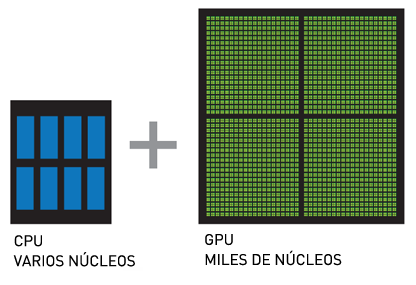
\includegraphics[width=0.8\textwidth]{img/cpu_gpu}
                 \caption{GPU and CPU core scheme}
                 \label{fig:core-scheme}
             \end{figure}
        \end{column}
    \end{columns}
\end{frame}

\subsubsection{Programming strategy}
\begin{frame}
    \frametitle{Computational Aspects}
    \framesubtitle{Programming strategy}

    \begin{columns}
        \begin{column}{0.5\textwidth}
            \begin{figure}
                \captionsetup{singlelinecheck=off}
                \centering
                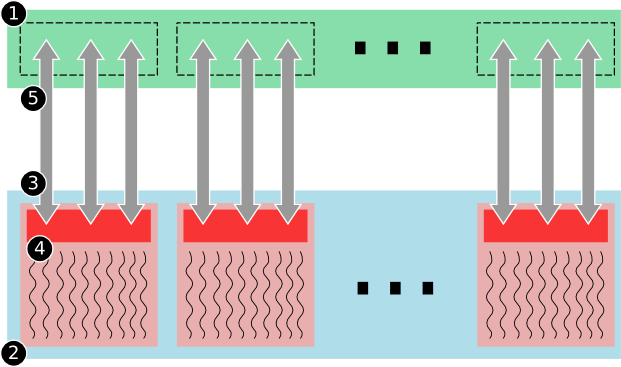
\includegraphics[width=0.9\textwidth]{img/cuda-strategy}
                \label{fig:estrategia}
                \caption{CUDA Programming strategy}
            \end{figure}
        \end{column}
        \begin{column}{0.5\textwidth}
             \begin{enumerate}
                 \item CPU memory allocation,
                 \item \dgreen{GPU} memory allocation,
                 \item Data copying,  CPU $\rightarrow$ \dgreen{GPU},
                 \item Task execution on the data,
                 \item Data copying, \dgreen{GPU} $\rightarrow$ CPU,
             \end{enumerate}
        \end{column}
    \end{columns}
\end{frame}
